\begin{enumerate}[label=\thechapter.\arabic*,ref=\thechapter.\theenumi]
\numberwithin{equation}{enumi}
\numberwithin{figure}{enumi}
\numberwithin{table}{enumi}

\item \begin{figure}[!ht]
    \centering
    \begin{circuitikz}
   \draw(0,0) to [R](2,0);
   % \draw (2,0) -- (2.5,0);
   \draw(2,0) to [L] (4,0);
   % \draw (5,0) to (5,0);
   \draw (4,0) to [C] (4,-2);
   \draw(4,-2)  to (0,-2);
   \draw (4,0) -- (5,0);
   \draw (4,-2)to (5,-2);
   \node[circle,fill,inner sep=1pt] at (0,0) {};
   \node[circle,fill,inner sep=1pt] at (5,0) {};
   \node[circle,fill,inner sep=1pt] at (5,-2) {};
   \node[circle,fill,inner sep=1pt] at (0,-2) {};
   \draw[->](0,-1.85) to (0,-0.15);
   \draw[->](5,-1.85) to (5,-0.15);
   \node at (0.3,-1) {$x(t)$};
   \node at (5.5,-1) {$y(t)$};

   \node at (1,0.5) {$R$};
   \node at (3,0.5) {$L$};
   \node at (2.8,-1) {$C$};\node[circle,fill,inner sep=1pt] at (0,0) {};
\end{circuitikz}

    \caption{RLC Low pass filter}
\end{figure}
The frequency response $y_{ss}(t)$ is defined as the steady state response to a sinusoidal input signal $x(t) = \sin{\omega t}$. It describes how well the filter can distinguish between different frequencies.
\begin{align}
y_{ss}(t)=\abs{H(j\omega)}\,\sin(\omega t+\angle H(j\omega))
\end{align}
\begin{enumerate}
    \item Overdamped Case
    \begin{align}
        H(s)=\omega_0^2\frac{1}{(s-p_1)(s-p_2)}
    \end{align}
    where,
    \begin{align}
        p_{1,2} &= -\frac{R}{2L} \pm \sqrt{\left(\frac{R}{2L}\right)^2-\frac{1}{LC}}\\
         H(s) &= \abs{H(s)}\ e^{j\angle{H(s)}}\\
         \abs{H(s)} &= \omega_0^2 \frac{1}{\abs{s-p_1}\abs{s-p_2}}\\
         &=\omega_0^2\frac{1}{\left|j\omega-p_2\right|\,\left|j\omega-p_2\right|} \\
         &= \omega_0^2 \frac{1}{\sqrt{\omega^2+{p_1}^2}\sqrt{\omega^2+{p_2}^2}}\\
         \angle H(s) &= -(\angle(s-p_1)+\angle(s-p_2))\\
         &= \tan^{-1}\frac{\omega}{p_1} + \tan^{-1}\frac{\omega}{p_2}
    \end{align}
    The magnitude of the transfer function expressed on a logarithmic scale:
    \begin{multline}
        \abs{H_{dB}(\omega)} = 20\log(\omega_0^2) -20\log\sqrt{\omega^2+{p_1}^2}  \\
        -20\log\sqrt{\omega^2+{p_2}^2}
    \end{multline}

    \item Critically damped case
    \begin{align}
        H(s)=\omega_0^2\frac{1}{(s-p)^2}
    \end{align}
    where,
    \begin{align}
        p &=\sqrt{\frac{1}{LC}}\\
        H(s) &= \abs{H(s)}\ e^{j\angle{H(s)}}\\
        \abs{H(s)} &= \omega_0^2 \frac{1}{\abs{s-p}^2}\\
        \abs{H(j\omega)} &=\omega_0^2 \frac{1}{\abs{j\omega-p}^2}\\
        &=\omega_0^2\frac{1}{\omega^2+p^2}\\
        \angle H(s) &= -(\angle(s-p)+\angle(s-p))\\
         &= 2\tan^{-1}\frac{\omega}{p}
    \end{align}
    The magnitude of the transfer function expressed on a logarithmic scale:
    \begin{align}
        \abs{H_{dB}(\omega)} = 20\log(\omega_0^2) -20\log(\omega^2+{p}^2)
    \end{align}

    \item Underdamped Case
    \begin{align}
        H(s)=\omega_0^2\frac{1}{(s-p)(s-p^\ast)}
    \end{align}
    where,
    \begin{align}
        p,\,p^\ast &=\omega_n\brak{-\zeta \pm j\sqrt{1-\zeta^2}}\\
        &= -\sigma\pm j\omega_d\\
        H(s) &= \abs{H(s)}\ e^{j\angle{H(s)}}\\
        \abs{H(s)} &= \omega_0^2\frac{1}{\sqrt{({\omega_n}^2-\omega^2)^2+(2\zeta\omega_n \omega)^2}}\\
        \angle H(s) &= -(\angle(s-p)+\angle(s-p^*))\\
         &= -\tan^{-1}\frac{\omega+\omega_d}{\sigma} - \tan^{-1}\frac{\omega-\omega_d}{\sigma}
    \end{align}
    The magnitude of the transfer function expressed on a logarithmic scale:
    \begin{multline}
        \abs{H_{dB}(\omega)} = 20\log(\omega_0^2) \\-10\log(({\omega_n}^2-\omega^2)^2+(2\zeta\omega_n \omega)^2)
    \end{multline}
\end{enumerate}
\begin{figure}[!ht]
    \centering
    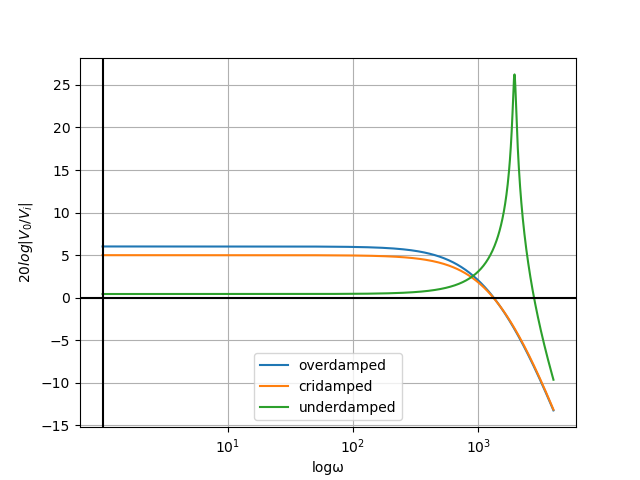
\includegraphics[width=\columnwidth]{app/figs/h_db_plot.png}
    \caption{Frequency response of all cases}
\end{figure}

\begin{figure}[!ht]
    \centering
    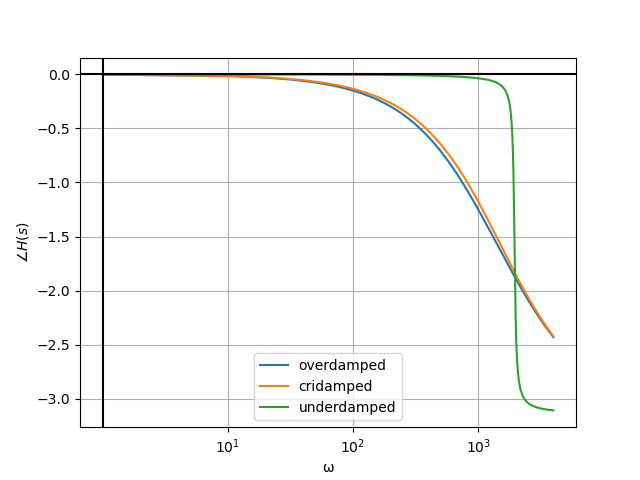
\includegraphics[width=\columnwidth]{app/figs/angle_H_s.png}
    \caption{Plot of $\angle H(s)$}
\end{figure}

\end{enumerate}
